\section{Photosensor System}
\label{sec:dp-pds-photosensors}

The baseline photodetector for the light readout is the Hamamatsu R5912-MOD20 \dword{pmt}. This is the same model used in \dword{pddp}. The Hamamatsu R5912-MOD20, depicted in  Figure~\ref{fig:dppd_2_1}, is an 8-inch diameter, 14-stage, high gain \dword{pmt} (nominal gain of \num{e9}). The maximum quantum efficiency of the R5912-MOD20 \dword{pmt} is approximately \SI{20}{\%} at \SI{400}{\nano\m}. In addition, this \dword{pmt} was designed to work at cryogenic temperatures by adding a thin platinum layer between the photocathode and the borosilicate glass envelope to preserve the conductance of the photocathode at low temperatures. This particular \dword{pmt} has proved reliable in other cryogenic detectors. The same or similar \dwords{pmt} have successfully operated in other \lar experiments like MicroBooNE~\cite{microboone}, MiniCLEAN \cite{miniclean}, ArDM, ICARUS T600 \cite{icarus}, and \dword{pddp}~\cite{protoDUNDP-tdr}. Discussions with other manufacturers like Electron Tubes Limited (UK) \cite{electrontubeslim} and HZC (China) \cite{hzc} are on-going to include them in the program.

\begin{dunefigure}[Picture of the Hamamatsu R5912-MOD20 \dword{pmt}.]{fig:dppd_2_1}
{Picture of the Hamamatsu R5912-MOD20 \dword{pmt} \cite{hamamatsu-5912}.}
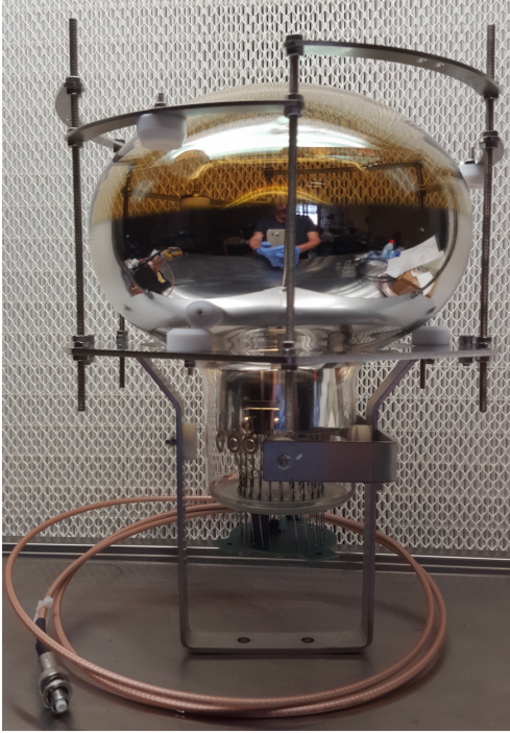
\includegraphics[width=0.3\textwidth]{dppd_2_1}
\end{dunefigure}

The baseline number of \dwords{pmt} is \dpnumpmtch with \num{80} spares.  Several operations and tests must be performed with the \dwords{pmt} before they are installed. The \dwords{pmt} must be ordered with sufficient lead time to complete the following planned operations: assembling the voltage divider circuit, mounting on the support structure, testing at room and cryogenic temperatures, packing and shipping to the \dword{ctsf}. The \dword{tpb} coating of the \dword{pmt} windows will be done at the \dword{ctsf}. The \dwords{pmt} will be re-tested for validation of basic functionality at the \dword{ctsf} and at \surf before installation (see Section~\ref{sec:dp-pds-installation}). Considering the large number of \dwords{pmt} required by \dual \dword{pds}, the purchase order must be completed at least two years before installation. A staged or staggered order with a steady supply of \dwords{pmt} would be most convenient and will be negotiated with the manufacturer.

%%%%%%%%%%%%%%%%%%%%%%%%%%%%%%%%%
\subsection{Photodetector Characterization}
\label{sec:dp-pds-selection-characterization}

Before installation, the most important characteristics of the \dword{pmt} response must be determined with two goals: to possibly reject under-performing \dwords{pmt} and to store the characterization information in a database for later use during the \dword{dpmod} commissioning and operation.

The basic and most important parameters to characterize are the dark count rate versus high voltage and the gain versus high voltage. Both parameters must be measured at room and cryogenic temperatures. As with the baseline \dword{pmt} model, the rates of pre-pulsing and after-pulsing should be negligible, but they will be measured as part of testing. 

From the mechanical point of view, the test set up requires a light-tight dark vessel filled with cryogenic liquid (argon or nitrogen) and an infrastructure for filling and operating the vessel with temperature and liquid-level controls. For \dword{pddp}, \num{10} \dwords{pmt} were tested at a time over a week because cryogenic tests of \dwords{pmt} require several days for \dword{pmt} thermalization \cite{Belver:2018erf}. Figure~\ref{fig:dppd_2_2a} shows the  \dword{pddp} \dwords{pmt} being installed in the testing vessel.
Increasing the capacity of the vessel, and thus the number of \dwords{pmt} that can be tested simultaneously,
could reduce the duration of the characterization test per \dword{pmt}.

\begin{dunefigure}[Picture of the \dwords{pmt} being installed in the testing vessel]{fig:dppd_2_2a}
{Picture of the \dwords{pmt} being installed in the testing vessel used for the \dword{pddp} \dwords{pmt}.}
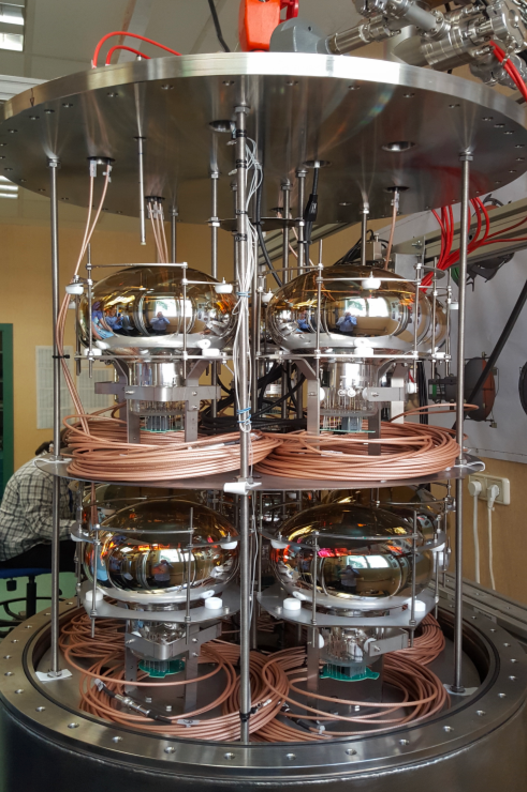
\includegraphics[width=0.3\textwidth]{dppd_2_2a}
\end{dunefigure}

Figure~\ref{fig:dppd_2_2b} shows a sketch of the proposed set up for \dword{pmt} characterization tests. For the electronics, the test set up requires an \dword{hv} power supply, a discriminator, a counter for the dark rate measurements, a pulsed light source, and a charge-to-digital or analog-to-digital converter for the \dword{pmt} gain versus voltage measurements. All instruments must allow computer control to automate data acquisition.

\begin{dunefigure}[Sketch of the set up for \dword{pmt} characterization tests.]{fig:dppd_2_2b}
{Sketch of the set up for \dword{pmt} characterization tests.}
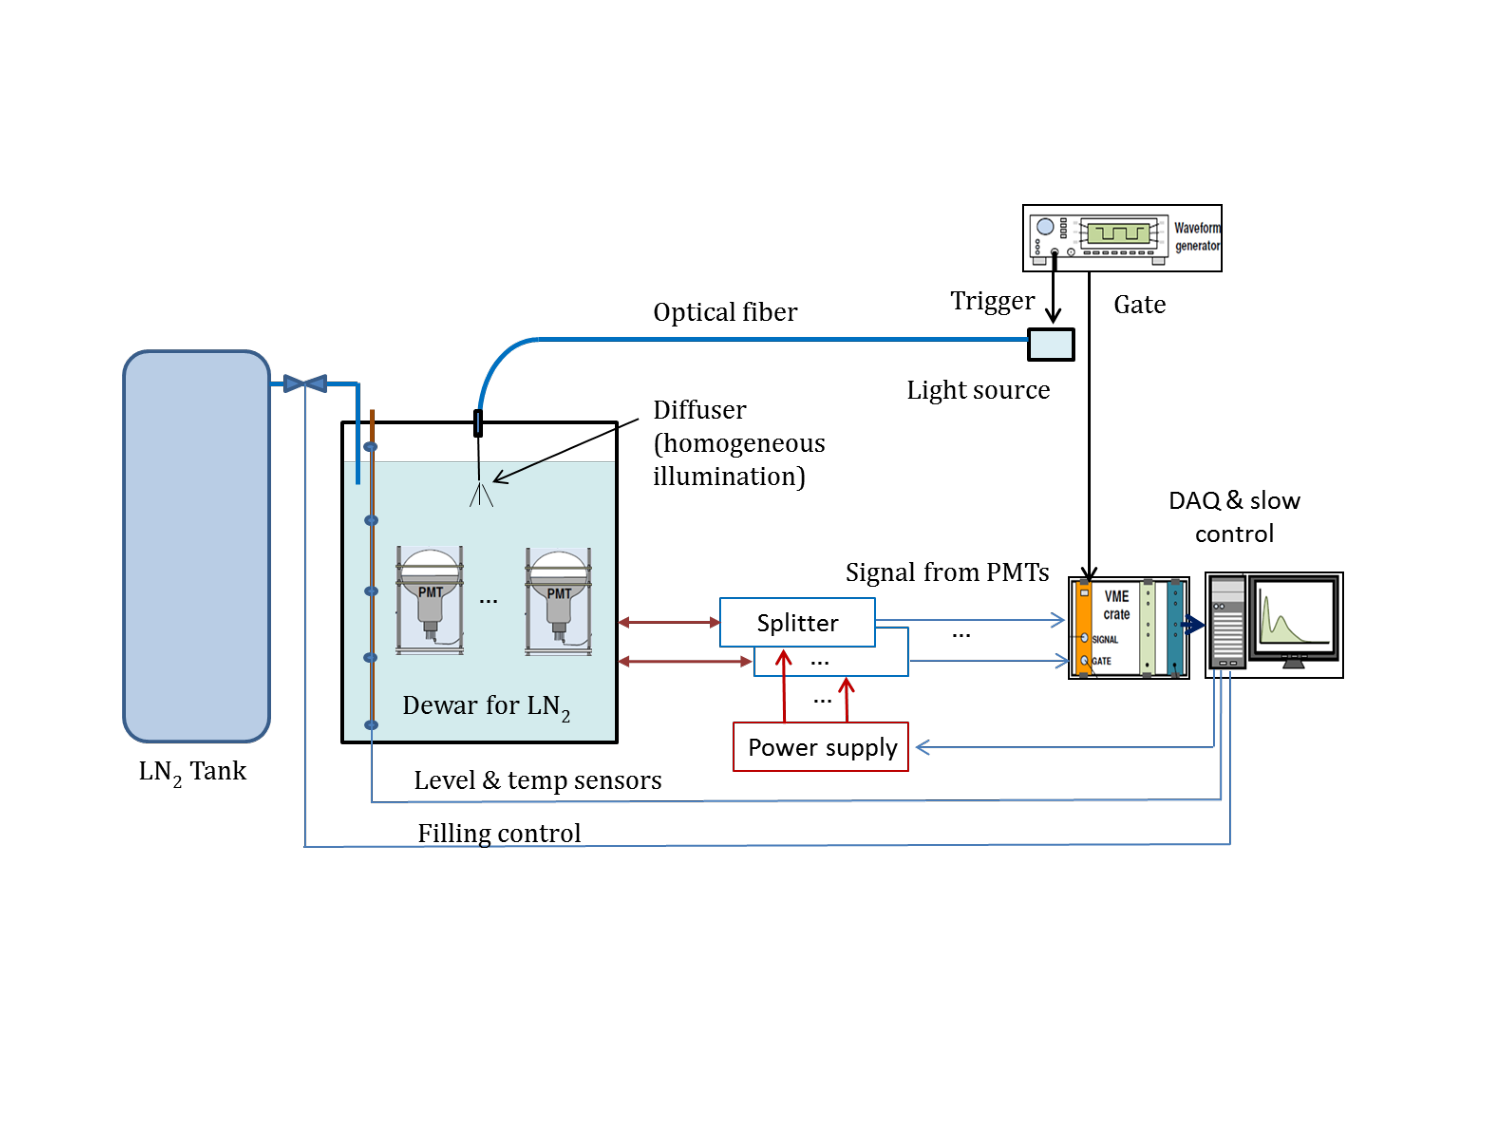
\includegraphics[width=0.7\textwidth]{dppd_2_2b}
\end{dunefigure}


%%%%%%%%%%%%%%%%%%%%%%%%%%%%%%%%%
\subsection{High Voltage System}
\label{sec:dp-pds-HV}

Based on the experience with the \dword{wa105} prototype, the A7030 power supply modules from CAEN~\footnote{CAEN\texttrademark{}, \url{http://www.caen.it/csite/CaenFlyer.jsp?parent=222}} are selected as the baseline power supply of the \dword{pmt} \dword{hv} system. 
These modules provide up to \SI{3}{kV} with a maximal output current of \SI{1}{mA} and a common floating ground to minimize noise. Module versions with \num{12}, \num{24}, \num{36}, or \num{48} \dword{hv} channels are available. The \dword{hv} polarity can be chosen for each module. Using the baseline \dword{pmt} powering scheme, modules with positive \dword{hv} polarity will be acquired for the experiment. Modules with \num{36} \dword{hv} channels and Radiall \num{52}\footnote{Radiall\texttrademark{}, \url{https://www.radiall.com/}.}  connectors are under consideration. The corresponding \dword{hv} cable connects the modules with the \dword{hv} splitters, described in Section~\ref{sec:fddp-pd-4.2}. For \dpnumpmtch \dwords{pmt}, \num{20} A7030 modules (+ \num{2} spares) are needed. These \num{20} \dword{hv} modules will be installed in mainframes from CAEN.

Each \dword{pmt} is powered individually.  This allows the gain of all \dwords{pmt} to be set individually by adjusting their operating high voltage.
This will be controlled by software. The software will interface to the \dword{pmt} calibration system and its database to extract the gain curves needed to set and/or equalize gains.

%%%%%%%%%%%%%%%%%%%%%%%%%%%%%%%%%
\subsection{Wavelength Shifting}
\label{sec:dppd-wls}

The \dual \dword{pds} requires wavelength-shifting of the \SI{127}{nm} scintillation photons toward visible wavelengths that can overlap with the photocathode luminous sensitivity. Coating the \dword{pmt} glass bulbs over the photocathode area with a thin film of \dword{tpb}  has already been validated~\cite{tpb} and is adopted as the baseline plan. 

\dword{tpb} is a wavelength shifter that has high efficiency for converting \lar scintillation \dword{vuv} light toward the light for which the \dword{pmt} photocathode is more sensitive. 

A thin layer of \dword{tpb} is deposited on the \dword{pmt} glass by means of a thermal evaporator that consists of a vacuum chamber with two copper crucibles (Knudsen cells) placed at the bottom of the chamber, see Figure~\ref{fig:dppd_11_4} in Section~\ref{sec:dp-pds-installation}. A \dword{pmt} is mounted on a rotating support that ensures a uniform coating layer and placed at the top of the evaporator with the  \dword{pmt} window pointing downward. The crucibles, filled with the \dword{tpb}, are heated to \SI{220}{\degreeCelsius}. At this temperature, the \dword{tpb} evaporates through a split in the crucible lid into the vacuum chamber, eventually reaching the \dword{pmt} window.

Several tests were performed to tune the evaporator's parameters, e.g., the coating thickness (\dword{tpb} surface density) and the deposition rate. A \dword{pmt} mock up covered with mylar foils was used for these tests. A \dword{tpb} surface density of \SI{0.2}{mg/cm^2}, the value for which the \dword{pmt} efficiency is stable as a function of the surface density, was chosen for \dword{pddp}. Efficiency measurements were performed by using a \dword{vuv} monochromator and by comparing the cathode current of a coated \dword{pmt} with the current value of a calibrated photodiode. From these efficiency tests, we concluded that approximately \SI{0.8}{g} of \dword{tpb} must be placed in the crucible for each evaporation to achieve the desired \dword{pmt} coating surface density. %The best deposition rate was fixed to about 6.5\,\AA/s. 
This value optimizes the quantity of \dword{tpb} used per evaporation while keeping the coating surface density fluctuations below \num{5}$\%$.  
Two to four \dwords{pmt}  with these specifications can be coated per day at a single coating station. 
Several coating stations will be required to keep the installation and testing schedule (see Section~\ref{sec:dp-pds-installation} for details). An average quantum efficiency of \SI{12}{\%} at \SI{127}{\nano\m} has been measured for TPB-coated \dwords{pmt} \cite{Bonesini:2018ubd}.

%We are considering, in coordination with the \dword{hvs} consortium, installing wavelength shifting films on the inner surfaces of the \dword{fc}. This would increase both light yield and response uniformity and is routinely used in \dual \lartpc{}s searching for dark matter, such as the ArDM~\cite{Boccone:2009zz} experiment. It is also under investigation for the \dword{spmod} concept, building on the experience of the \lariat experiment and the design for SBND. The same \dword{wls} compound used to coat the \dword{pmt} windows, \dword{tpb}, could be vacuum-evaporated on foils. The shifted longer wavelength light emitted by the foils would have a better chance to reach the \dword{pmt} windows than \SI{127}{nm} light because it has better reflective properties. 
 %
 %This concept would need to be demonstrated satisfactorily for performance and stability on the timescale of the experiment duration before it could become a part of the \dword{pds} system.

In order to enhance the light collection and to improve the photon detector response uniformity throughout the entire \dword{tpc} active volume, \dword{tpb} coated reflector/\dword{wls} panels will be installed on the \dword{fc} inner surfaces. The impact on the light yield and physics measurements was evaluated for two particular cases: The full coverage of the \dword{fc} inner walls with the panels and the coverage of only the upper half of the \dword{fc}. The conclusion from the simulation studies is that half coverage is sufficiently performant as shown in Fig. ~\ref{fig:dppd_fd_light_yield_comparisons}. In order to reduce the cost still keeping the \dword{pds} response uniformity, the baseline design is to equip only the top half of the \dword{fc} walls.

The reflector/\dword{wls} panel will be constructed with \SI{1}{\mm} thick \SI{93}{\cm} $\times$ \SI{93}{\cm} G10/FR4 plates. The central \SI{91}{\cm} (H) $\times$ \SI{93}{\cm} (W) area only on one side of the panel will be laminated with a reflective foil, which will then be evaporated with \dword{tpb}. The top and bottom \SI{1}{\cm} portion of the panel without coated foils will be sandwiched between horizontal support bars. Sketches of the panel are shown in Fig.~\ref{fig:dppd_reflective_panel}. The support structure of the panels is described in Section~\ref{sec:dp-pds-mechanics}. 
\begin{dunefigure}[Sketches of the front (left) and side (right) views of the reflective foil/\dword{wls} panel.]{fig:dppd_reflective_panel}
{Sketches of the front (left) and side (right) views of the reflector/\dword{wls} panel (not to scale).}
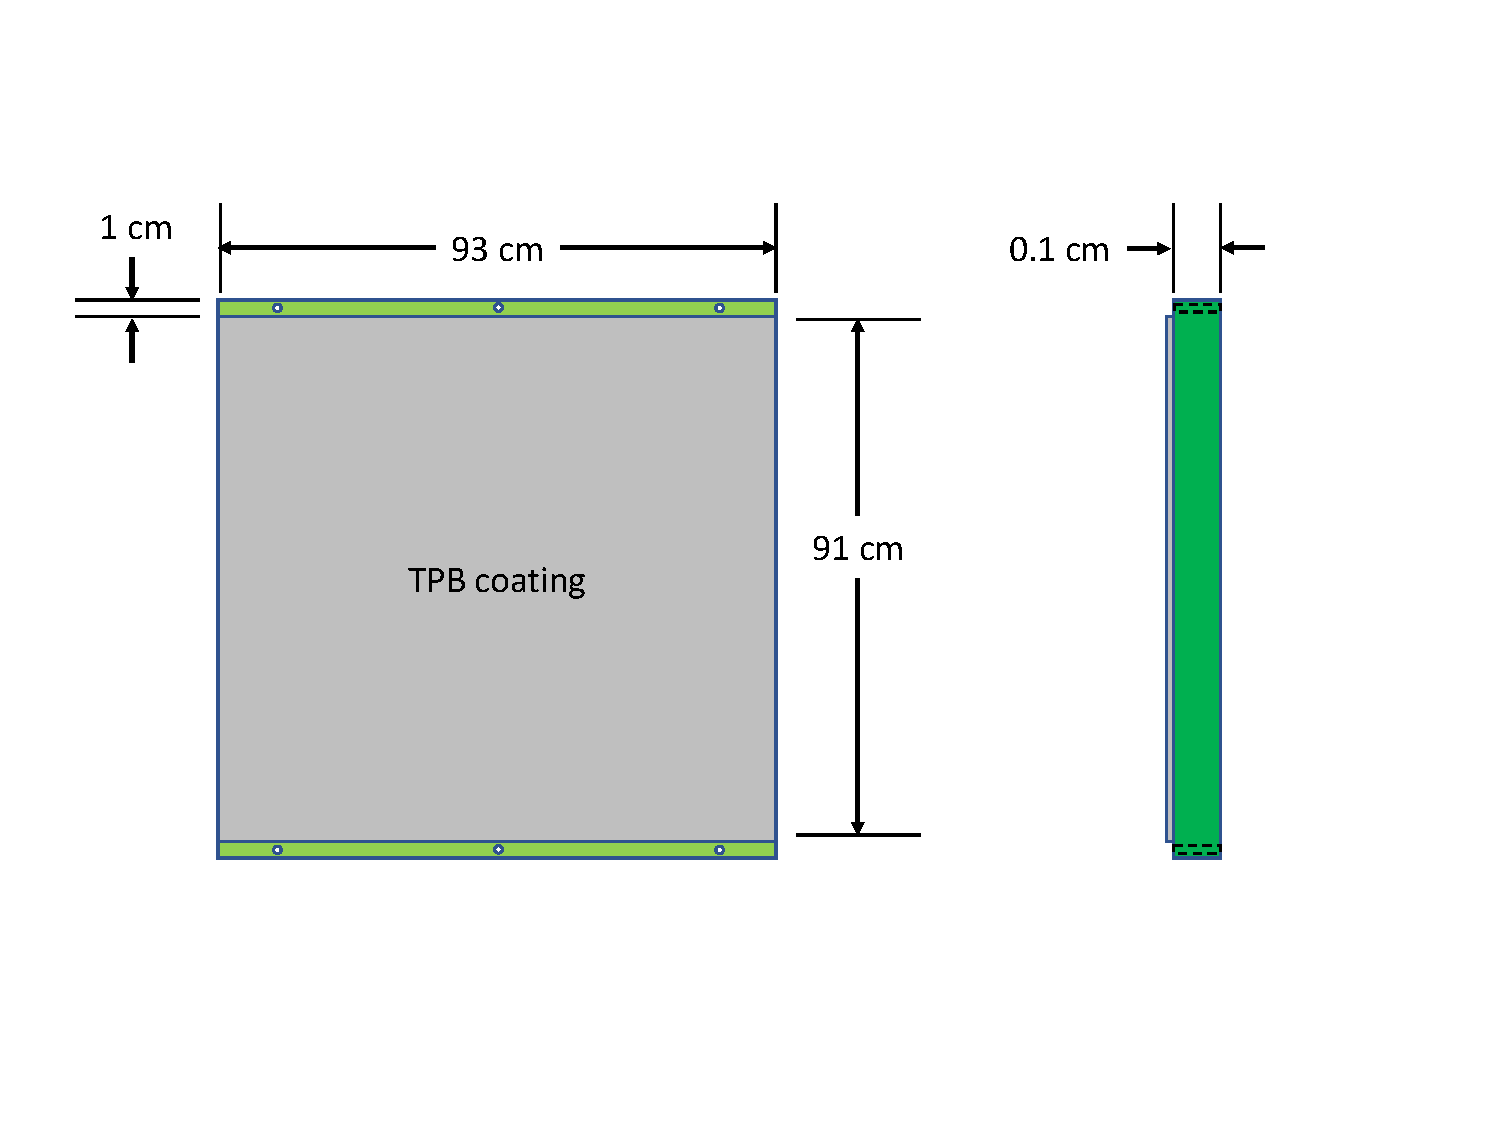
\includegraphics[width=0.7\textwidth]{dppd_reflective_panel}
\end{dunefigure}
